\documentclass[11pt]{article}
\usepackage[a4paper,margin=2cm]{geometry}
\title{%
    The Hare and the Tortoise \\
    \large A mini project \\
}
\author{Patrick Pellacani Muller}
\setcounter{section}{-1}

\usepackage{siunitx}
\usepackage{minted}

% tikz setup
\usepackage{tikz}
\usetikzlibrary{positioning,shapes.geometric,arrows.meta}

\tikzstyle{startstop} = [rectangle, rounded corners, minimum width=3cm, minimum height=0.8cm, text centered, draw=black, fill=gray!20, font=\small]
\tikzstyle{process} = [rectangle, minimum width=3cm, minimum height=0.8cm, text centered, draw=black, fill=gray!10, font=\small]
\tikzstyle{decision} = [diamond, aspect=2, text centered, draw=black, fill=gray!10, font=\small, inner sep=3pt]
\tikzstyle{io} = [trapezium, trapezium left angle=70, trapezium right angle=110,
                   minimum width=3cm, minimum height=0.8cm, text centered, draw=black, fill=gray!10, font=\small]
\tikzstyle{subprog} = [
    rectangle, minimum width=3cm, minimum height=0.8cm,
    text centered, draw=black, fill=gray!5, font=\small,
    inner xsep=8pt,
    path picture={
        \draw[line width=0.8pt]
            ([xshift=0.15cm]path picture bounding box.north west) --
            ([xshift=0.15cm]path picture bounding box.south west);
        \draw[line width=0.8pt]
            ([xshift=-0.15cm]path picture bounding box.north east) --
            ([xshift=-0.15cm]path picture bounding box.south east);
    }
]
\tikzstyle{arrow} = [thick, ->, >=Stealth]
\tikzstyle{structnode} = [
    rectangle,                 % Shape
    draw=black,                % Border color
    thick,                     % Slightly thicker border
    rounded corners=2pt,       % Optional: slightly rounded
    minimum width=2cm,       % Width
    minimum height=1cm,        % Height
	inner xsep=5pt,
    text centered,             % Centered text
    fill=gray!15,              % Subtle background
    font=\small                % Font size
]



\usepackage{datetime}
\newdate{writing_date}{13}{10}{2025}
\date{\displaydate{writing_date}}

\usepackage{biblatex}
\addbibresource{sources.bib}

\begin{document}
\maketitle
\section{Introduction}
\subsection{Purpose}
The main purpose of the program is entertainment as it is a game to be enjoyed. It
simulates the classic story of the tortoise and the hare. To make the game enjoyable,
the user is asked to bet on either the hare or the tortoise. This money is then used
to play another round as long as the user has enough money. The more rounds a user
is able to play, the better their final score.
\subsection{Intended user}
Possible users of the program are younger children as the game loop is very simple and
may not appeal as much to older children, teenagers or adults. It should therefore be easy
to use and understand. However, there may be moral considerations when aiming a game that
involves gambling and betting to (young) children. This is combated by using the artificial
currency of "carrots" which the user can use to bet on an animal. If they win, they gain
"carrots". The aim of the game is therefore not to make the most money gambling but instead
to collect the most "carrots" in a given number of rounds to feed \cite{hare-diet,tortoise-diet}
the animals. The animals require feeding to play another round.
\subsection{Functionality}
A simple pseudo-random number generator based simulation of the game of ``the hare and the
tortoise''. The initial parameters for the simulation are:
\begin{itemize}
	\item The game is divided into rounds, and finishes when the first person reaches
	      \qty{1000}{\metre}
	\item Each round the tortoise moves \qtyrange{5}{10}{\metre}
	\item Each round the hare moves \qtyrange{8}{15}{\metre}
	\item However, there is a \qty{25}{\percent} chance that the hare doesn't move
\end{itemize}

The betting system has odds set out to increase the user's "carrots" slightly if the fee for
playing a new round is not taken into account. However, as there is a fee to play each round,
on average, the number of carrots that a player has tends to zero. More on the specific carrot
mechanic in the Betting section.

\subsection{Why a computational approach was used}
\label{sec:approach}
A computational approach is best here as the races can be quite long and can be simulated more
quickly. As the game is aimed at children, a lengthy process of e.g. rolling dice may be unrealistic
as most children will be bored before the first game even finishes. For example, on average the
tortoise would take \(\frac{1000}{7.5} \approx 134\) rounds to complete a race. Assuming a dice roll
every \qty{2}{\second}, this will take
\(134 \times \qty{2}{\second} = \qty{268}{\second} \approx \qty{4.5}{\minute}\) of dice rolls.

The programming language that is used in this project is Rust \cite{rust} which provides a
safe, compiled language. The main reasons for this is to offer security and help with data
validation. By having using a compiled language, the program will run more efficiently, which
isn't a major concern right now but allows for a better integration of a more complex UI and
game mechanics later. Furthermore, the game is aimed at children who often do not have the money to
buy powerful PCs, and performance could be a major factor later if new features get added.
From a development point of view, using Rust allows for the use of modern tools such as functional
programming to keep code neat, tidy, legible and extensible.

\section{Data structures}
The constants used in the program are defined in Table~\ref{tab:consts}, and the variables
in Table~\ref{tab:vars}. Four custom structs as well as one enum are used for modularity, and
their relationship as well as structure can be seen in Figure~\ref{fig:structs}.

The decision to make \texttt{Animal} an enum has the upside of allowing the addition of  more animals
while minimizing the risk that the new animals aren't properly implemented in code as Rust ensures that
all enum elements are covered whenever one is using enums. This improves the program's extensibility
greatly.

The four structs used allow the code to stay segmented and modular, therefore allowing a team of
developers to work on the project simutaneously. When winning is being implemented, one doesn't have
to think about how the betting mechanic works, and instead leave that up to the \texttt{Bet} struct
to hanlde. This improves efficiency when developing and allows for greater extensibility later in the
program's lifecycle.

\begin{table}[!ht]
	\centering
	\begin{tabular}{ | c c | }
		\hline
		Name                               & type              \\
		\hline
		\texttt{race\_length}              & \texttt{u32}      \\
		\texttt{tortoise\_speed\_interval} & \texttt{Interval} \\
		\texttt{hare\_speed\_interval}     & \texttt{Interval} \\
		\texttt{hare\_sleep\_chance}       & \texttt{f64}      \\
		\hline
	\end{tabular}
	\caption{Constants used in the game}%
	\label{tab:consts}
\end{table}
\begin{table}[!ht]
	\centering
	\begin{tabular}{ | c c | }
		\hline
		Name              & type                 \\ \hline
		\texttt{hare}     & \texttt{Hare}        \\
		\texttt{tortoise} & \texttt{Tortoise}    \\
		\texttt{winners}  & \texttt{WinnerTable} \\
		\texttt{money}    & \texttt{f64}         \\
		\texttt{bet}      & \texttt{Bet}         \\ \hline
	\end{tabular}
	\caption{Variables used in the game}
	\label{tab:vars}
\end{table}

\begin{figure}[!ht]
	\centering
	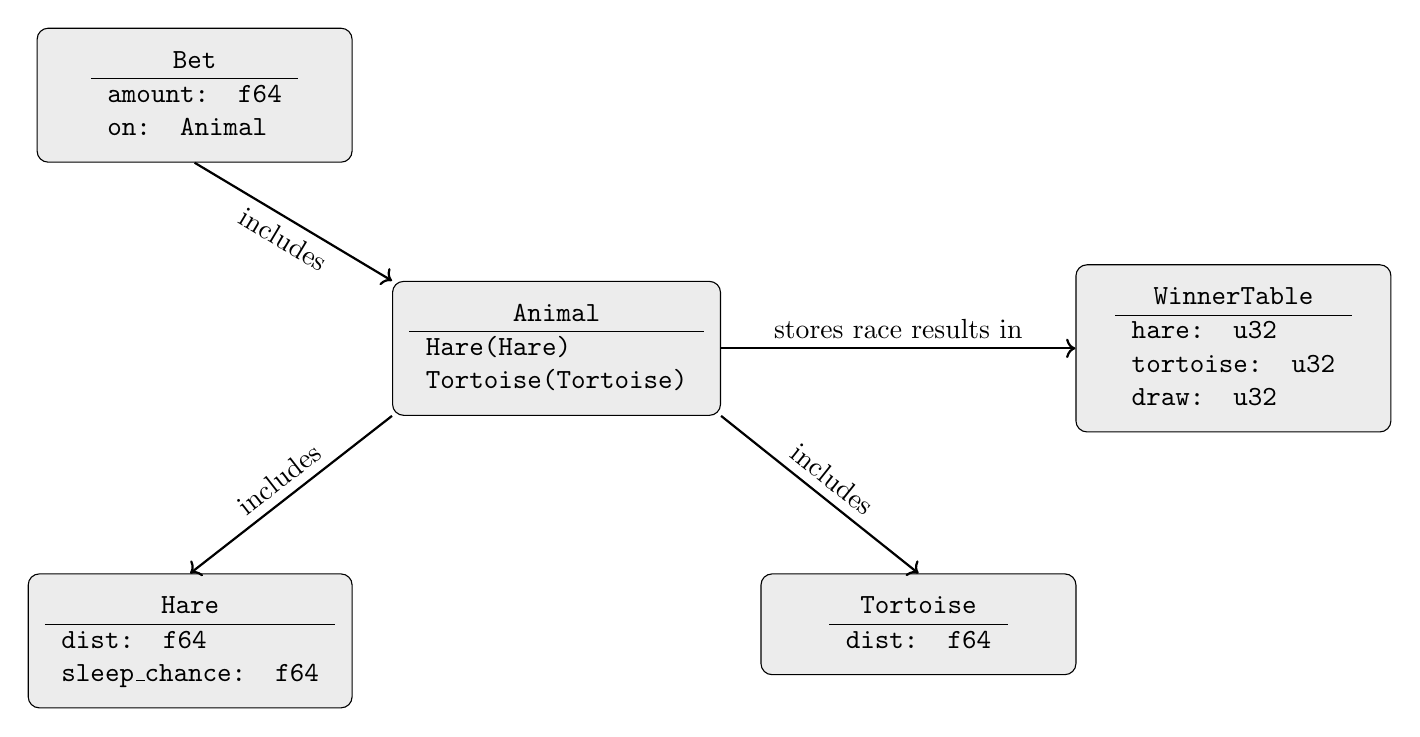
\begin{tikzpicture}[
			struct/.style={
					rectangle,
					draw=black,
					rounded corners,
					fill=gray!15,
					minimum width=4cm,
					inner sep=6pt,
					font=\ttfamily,
				}
		]

		% Animal enum
		\node[struct] (animal) {
			\begin{tabular}{l}
				\multicolumn{1}{c}{Animal} \\ \hline
				Hare(Hare)                 \\
				Tortoise(Tortoise)         \\
			\end{tabular}
		};

		% Hare struct
		\node[struct, below left=2cm and 0.5cm of animal] (hare) {
			\begin{tabular}{l}
				\multicolumn{1}{c}{Hare} \\ \hline
				dist: f64                \\
				sleep\_chance: f64       \\
			\end{tabular}
		};

		% Tortoise struct
		\node[struct, below right=2cm and 0.5cm of animal] (tortoise) {
			\begin{tabular}{l}
				\multicolumn{1}{c}{Tortoise} \\ \hline
				dist: f64                    \\
			\end{tabular}
		};

		% WinnerTable struct
		\node[struct, right=4.5cm of animal] (winner) {
			\begin{tabular}{l}
				\multicolumn{1}{c}{WinnerTable} \\ \hline
				hare: u32                       \\
				tortoise: u32                   \\
				draw: u32                       \\
			\end{tabular}
		};

		% Bet struct
		\node[struct, above left=1.5cm and 0.5cm of animal] (bet) {
			\begin{tabular}{l}
				\multicolumn{1}{c}{Bet} \\ \hline
				amount: f64             \\
				on: Animal              \\
			\end{tabular}
		};

		% Connections
		\draw[->, thick] (animal.east) -- node[above,sloped]{stores race results in} (winner.west);
		\draw[<-, thick] (hare.north) -- node[above,sloped]{includes} (animal.south west);
		\draw[<-, thick] (tortoise.north) -- node[above,sloped]{includes} (animal.south east);
		\draw[->, thick] (bet.south) -- node[below,sloped]{includes} (animal.north west);

	\end{tikzpicture}
	\caption{The structure diagram of the \texttt{struct}s \texttt{Hare}, \texttt{Tortiose}}
	\label{fig:structs}
\end{figure}

\section{Outline of Program}
\subsection{Overview of main algorithm}
The flowchart in Figure~\ref{fig:flw-prgm} outlines clearly the main program loop and how the main
part of the program calls the smaller modules. Below, the same idea, written in pseudocode, can be found.
\begin{listing}
	\begin{minted}[frame=lines]{text}
        DO
            bet := setup_bet(Input("How much to bet?"), Input("Betting on tortoise or hare"))
            WHILE NOT race_ended()
                move_animals()
            ENDWHILE
            announce_winner()
            store_winner()
            calculate_bet()
        WHILE Input("Another Race?")
        output_stats()
        \end{minted}
	\caption{A pseudocode overview of the main program.}
	\label{lst:psd-overview}
\end{listing}
\begin{figure}[!ht]
	\centering
	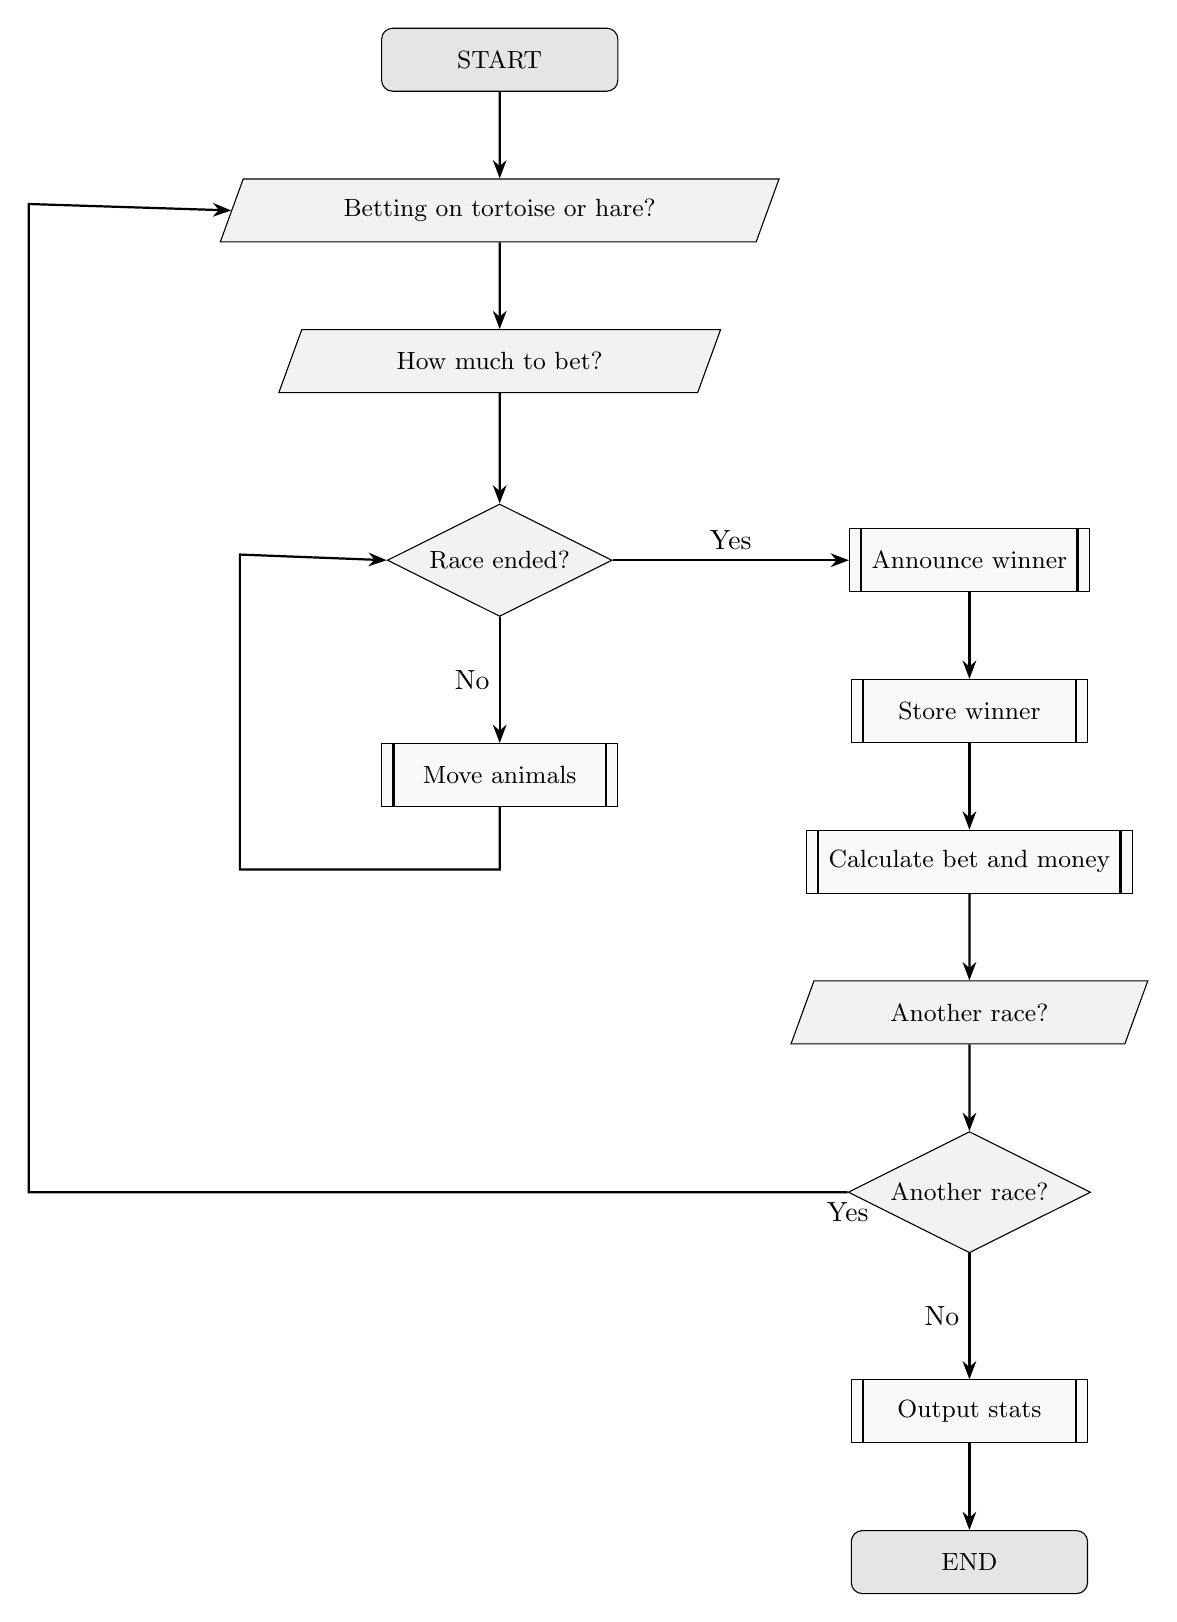
\begin{tikzpicture}[node distance=1.1cm]

		% Nodes
		\node (start) [startstop] {START};
		\node (betchoice) [io, below=of start] {Betting on tortoise or hare?};
		\node (betamt) [io, below=of betchoice] {How much to bet?};

		\node (racecheck) [decision, below=of betamt, yshift=-0.3cm] {Race ended?};
		\node (move) [subprog, below=of racecheck, yshift=-0.5cm] {Move animals};

		\node (announce) [subprog, right=3cm of racecheck] {Announce winner};
		\node (store) [subprog, below=of announce] {Store winner};
		\node (money) [subprog, below=of store] {Calculate bet and money};

		\node (again) [io, below=of money] {Another race?};
		\node (againcheck) [decision, below=of again] {Another race?};

		\node (stats) [subprog, below=of againcheck, yshift=-0.5cm] {Output stats};
		\node (stats) [subprog, below=of againcheck, yshift=-0.5cm] {Output stats};
		\node (stop) [startstop, below=of stats] {END};

		% Arrows
		\draw [arrow] (start) -- (betchoice);
		\draw [arrow] (betchoice) -- (betamt);
		\draw [arrow] (betamt) -- (racecheck);

		\draw [arrow] (racecheck) -- node[anchor=east] {No} (move);
		\draw [arrow] (move) -- ++(0,-1.2) -| ++(-3.3,4) -- (racecheck.west);
		\draw [arrow] (racecheck) -- node[anchor=south] {Yes} (announce);

		\draw [arrow] (announce) -- (store);
		\draw [arrow] (store) -- (money);
		\draw [arrow] (money) -- (again);
		\draw [arrow] (again) -- (againcheck);

		\draw [arrow] (againcheck) -- node[anchor=east] {No} (stats);
		\draw [arrow] (stats) -- (stop);
		\draw [arrow] (againcheck.west) node[anchor=north] {Yes} -- ++(-10.4,0) -- ++(0,12.55) -- (betchoice.west);
	\end{tikzpicture}
	\caption{Flowchart of the main program}
	\label{fig:flw-prgm}
\end{figure}
\subsection{Modularity}
\label{sec:modules}
\begin{figure}[!ht]
	\centering
	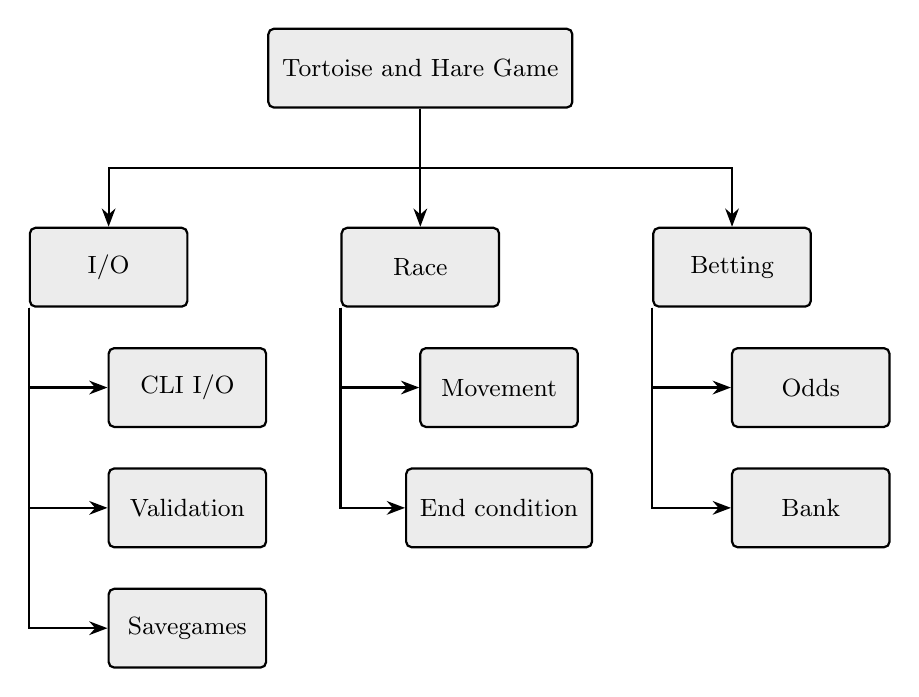
\begin{tikzpicture}[node distance=0.5cm]

		% Top-level module
		\node[structnode] (game) {Tortoise and Hare Game};

		% Input module
		\node[structnode, below left=1.5cm and 1cm of game] (io) {I/O};
		\node[structnode, below=of io, xshift=1cm] (cli_io) {CLI I/O};
		\node[structnode, below=of cli_io] (validation) {Validation};
		\node[structnode, below=of validation] (storage) {Savegames};


		% Race module
		\node[structnode, below=1.5cm of game] (race) {Race};
		\node[structnode, below=of race, xshift=1cm] (move) {Movement};
		\node[structnode, below=of move] (end) {End condition};

		% Statistics module
		\node[structnode, below right=1.5cm and 1cm of game] (bet) {Betting};
		\node[structnode, below=of bet, xshift=1cm] (odds) {Odds};
		\node[structnode, below=of odds] (bank) {Bank};

		% Arrows
		\draw[arrow] (game.south) -- ++(0,-0.75) -| (io);
		\draw[arrow] (io.south west) |- (cli_io);
		\draw[arrow] (io.south west) |- (validation);
		\draw[arrow] (io.south west) |- (storage);

		\draw[arrow] (game.south) -- ++(0,-0.75) -| (race);
		\draw[arrow] (race.south west) |- (move);
		\draw[arrow] (race.south west) |- (end);

		\draw[arrow] (game.south) -- ++(0,-0.75) -| (bet);
		\draw[arrow] (bet.south west) |- (bank);
		\draw[arrow] (bet.south west) |- (odds);
	\end{tikzpicture}
	\caption{Structure diagram outlining the main modules}

\end{figure}

\section{In-depth Gameplay analysis}


\section{Test data}
\subsection{Inputs and testing approach}
The main data inputs are:
\begin{itemize}
	\item Choosing between betting on the tortoise or hare
	\item Entering the amount of money to bet
	\item Deciding whether or not to play another round
\end{itemize}

Because Rust is used as the programming language (see Section~\ref{sec:approach}), data safety
and errors such as buffer overflow errors are dealt with by the language. However, testing that
these safeguards are in place properly is still good practice, especially as the default response
to such an error in Rust would be a ``\texttt{panic}'', which stops the program abruptly and may
instill annoyance in users if they experience such an error in the middle of the game.

To ensure the correct functionality of individual modules, unit testing will be used throughout
the development phase. This ensures that the individual modules outlined in Section~\ref{sec:modules}
are working as intended. The that is used for testing is outlined in Section ~\ref{sec:unit-test}

Furthermore, testing after development with valid, boundary, invalid and erroneous data will ensure
that the whole program works as expected. This data is outlined in Section~\ref{sec:whole-test}.
\subsection{Unit Testting}
\label{sec:unit-test}
\subsection{Validation Testing}
\label{sec:whole-test}
\section{Source code}
\section{Testing}
\section{Evaluation}
\end{document}
